\chapter{Appendix: how to set up the drone}\label{app:setup}
This appendix describes how to set up the drone to take off and it is useful for readers that are not that familiar with the Patmos architecture or that want to further develop the flight controller.
Most of the following sections show parts of scripts and commands that can be found on the Patmos Handbook \cite{bib:patmos_hnd} or in the support and complementary PREDICT repository \cite{bib:pred_repo}.

For the set up, it is necessary to use computer with Ubuntu 18 at least. In case of not having one, it is possible to use the Virtual Machine (VM) provided by the Patmos main webpage \cite{bib:patmos_page}.

On top of that, this project uses the multi-core feature, which needs the external memory on the microSD of the De10-Nano board. Before downloading Patmos on the board, it is necessary to flash the SD card in order to make it compatible with the system. Files available in \cite{bib:microSD} and detailed description on the README.md in the Quartus Prime project for de10-nano-drone.

\section*{Running Patmos on the board}
The model used in this project is the FPGA De10-Nano from Altera and the Patmos OS is implemented in a Quartus Prime project. To download it on the board from a computer, it is necessary to follow two processes: install Patmos dependencies on the computer and connect it to the board.

To install Patmos:
\begin{enumerate}
	\item Create a folder called "t-crest" on your home address.
	\item Download and rename the following repositories from the T-Crest project \cite{bib:tcrest_repo}.

\lstset{style=Bstyle}
\begin{lstlisting}[language=bash]
mkdir t-crest && cd ~/t-crest
git clone https://github.com/t-crest/aegean.git
git clone https://github.com/t-crest/argo.git 
git clone https://github.com/t-crest/patmos-compiler-rt.git compiler-rt
git clone https://github.com/t-crest/patmos-gold.git gold
git clone https://github.com/t-crest/patmos-llvm.git llvm
git clone https://github.com/t-crest/patmos-misc.git misc
git clone https://github.com/t-crest/patmos-newlib.git newlib
\end{lstlisting}

	\item Delete the previous build folders.

\begin{lstlisting}[language=bash]
rm -rf ~t-crest/newlib/build
rm -rf ~t-crest/patmos/hardware/build
\end{lstlisting}

	\item Re-build and compile the libraries

\begin{lstlisting}[language=bash]
cd misc
cp build.cfg.dist build.cfg
./build.sh
cd ..
./misc/build.sh newlib
cd patmos/doc
make
\end{lstlisting}
	
	\item Check if the commands are available.
\begin{lstlisting}[language=bash]
Still on process
\end{lstlisting}

    \item In case that Patmos has been updated (new features has been added, another model has been included, etc), it is necessary to update accordingly.
    
\begin{lstlisting}[language=bash]
cd ~/t-crest/
gitall pull
# Repite build and compilation process from here
\end{lstlisting}    

\end{enumerate}

To download Patmos on a de10-nano board for the first time, it is necessary to set up some additional configuration:
\begin{enumerate}
	\item Install the FPGA drivers on the computer. The drivers must be located on the /dev/ folder, in a file. It's possible either to copy the file \textit{51-usbblaster.rules} from the complementary repository\cite{bib:pred_repo} or generate it with the following content:
	
\lstset{style=OtherSt}
\lstinputlisting{Figures/setup/Files/51-usbblaster.rules} 	

	\item Give to the computer user account the right to access the communication ports.
	
\lstset{style=Bstyle}
\begin{lstlisting}[language=bash]
sudo usermod -a -G dialout user
# Now log out from the computer and sign in again
\end{lstlisting} 

	\item Connect a FPGA to the computer and check if it can be recognised.
	
\begin{lstlisting}[language=bash]
jtagconfig
# In case the command gets stuck, kill it and re-run it
sudo killall -9 jtagd
\end{lstlisting} 	

%\end{enumerate}

\begin{figure}[H]
    \centering
        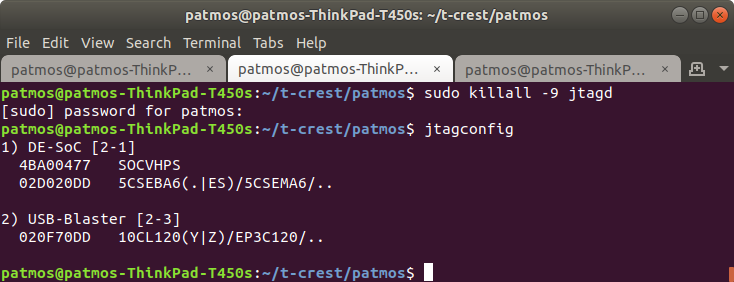
\includegraphics[scale=0.5]{Figures/setup/jtagconfig.png}
    \caption{Running the jtagconfig command shows every connected FPGA. In this case, it shows a de10-nano (De-SoC) on port 2-1 and a de2-115 (USB-Blaster) on port 2-3.}
    \label{fig:jtagconfig}
\end{figure}

Finally, to download the Quartus Prime project on the board it is necessary to compile the Patmos folders according to a certain model. Afterwards, the FPGA shall retain the architecture in its memory even after turning on and off. 
In case a C app does not run correctly, repeat only the last steps inside Quartus Prime. In case the issue still persists, repeat this procedure:
%\begin{itemize}
    \item Check that selected board is de10-nano-drone and that the communication type is DE-SoC. This is set up in the Makefile located in \textit{~/t-crest/patmos}:

\lstset{style=Bstyle}
\begin{lstlisting}[language=bash]
# Altera FPGA configuration cables
#BLASTER_TYPE=ByteBlasterMV
#BLASTER_TYPE=Arrow-USB-Blaster
BLASTER_TYPE?=DE-SoC 
#BLASTER_TYPE?=USB-Blaster

# The Quartus/ISE project
#BOARD=ml605oc
#BOARD=bemicro
#BOARD?=altde2-70
#BOARD?=altde2-115
BOARD?=altde10-NANO-oc
\end{lstlisting} 
    
    \item Check the hardware configuration for the de10-nano-drone. For this flight controller, four cores are required and the sensors are distributed and assigned between the different cores. The configuration can be checked on the \textit{~/t-crest/patmos/hardware/config/de10-nano-drone.xml}:
    
\lstset{style=Bstyle}
\begin{lstlisting}[language=bash]
<patmos default="default.xml">
  <description>Configuration for de10-nano board for drone with external ddr3 memory</description>

  <frequency Hz="50000000"/>
  <pipeline dual="false" />
  <cores count="4" />
  <ExtMem size="1g" DevTypeRef="DDR3Bridge" />

  <IOs>
  <IO DevTypeRef="Uart1" offset="6" core="3"/>
  <IO DevTypeRef="Uart2" offset="7" core="3"/>
  <IO DevTypeRef="Leds" offset="9" core="0"/>
  <IO DevTypeRef="I2CMaster" offset="11" core="1"/>
  <IO DevTypeRef="Actuators" offset="12" core="2"/>
  <IO DevTypeRef="SPIMaster" offset="14" core="0"/>
  </IOs>

  <Devs>
    <Dev DevType="Uart1" entity="Uart" iface="OcpCore">
      <params>
        <param name="baudRate" value="9600"/>
        <param name="fifoDepth" value="16"/>
      </params>
    </Dev>
    <Dev DevType="Uart2" entity="Uart" iface="OcpCore">
      <params>
        <param name="baudRate" value="115200"/>
        <param name="fifoDepth" value="128"/>
      </params>
    </Dev>
    <Dev DevType="Leds" entity="Leds" iface="OcpCore">
      <params>
        <param name="ledCount" value="8"/>
      </params>
    </Dev>
    <Dev DevType="I2CMaster" entity="I2CMaster" iface="OcpCore">
      <params>
        <param name="i2cBitRate" value="100000" />
      </params>
    </Dev>
    <Dev DevType="Actuators" entity="Actuators" iface="OcpCore">
      <params>
          <param name="extAddrWidth" value="16" />
          <param name="dataWidth" value="32" />
      </params>
    </Dev>

    <Dev DevType="SPIMaster" entity="SPIMaster" iface="OcpCore">
      <params>
          <param name="slaveCount" value="1" />
          <param name="sclk_scale" value="1" /> 
          <param name="fifoDepth" value="6"/>
          <param name="wordLength" value="12"/>
      </params>
    </Dev>

    <Dev DevType="DDR3Bridge" entity="DDR3Bridge" iface="OcpBurst" />
    <Dev DevType="OCRam" entity="OCRamCtrl" iface="OcpBurst">
      <params>
         <param name="sramAddrWidth" value="19" />
      </params>
    </Dev>
  </Devs>
</patmos>
\end{lstlisting}
    
    \item Compile Patmos for the de10-nano-drone set up. This can be done either all at once or per steps. In case of errors, it is recommended to do it per steps according to the Handbook\cite{bib:patmos_hnd} and check where the compilation fails.

\lstset{style=Bstyle}
\begin{lstlisting}[language=bash]
cd ~/t-crest/patmos
export BOARD=de10-nano-drone
rm -rf ~/t-crest/patmos/hardware/build
make gen
make -C hardware verilog BOOTAPP=bootable-bootloader BOARD=de10-nano-drone
make synth
\end{lstlisting} 
    
    \item Open Quartus Prime. The de10-nano-drone project is located in \textit{~/t-crest/patmos/} \textit{hardware} \textit{/quartus/de10-nano-drone/patmos.qpf}. In the case the project is not compiled yet, run "Compile Design" on the Task bar, to convert the project to a .sof binary file. 

\begin{figure}[H]
    \centering
        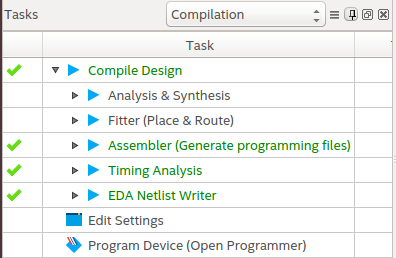
\includegraphics[scale=0.5]{Figures/setup/quatus_compile.png}
    \caption{If during the compilation in Quartus Prime errors were given, review the hardware settings, such as the board model, cores number, etc.}
\end{figure}

    \item By default, the compiled projects have the extension .sof and they are volatile, which means that after the FPGA is restarted, the Quartus project must be downloaded again. This is also an issue for using the multicore feature. To make the project permanent, it is necessary to convert the .sof into a .jic file. On Quartus Prime, go to \textit{Files/Convert Programming Files...} and generate the .jic file with the following options:
    
\begin{figure}[H]
    \centering
        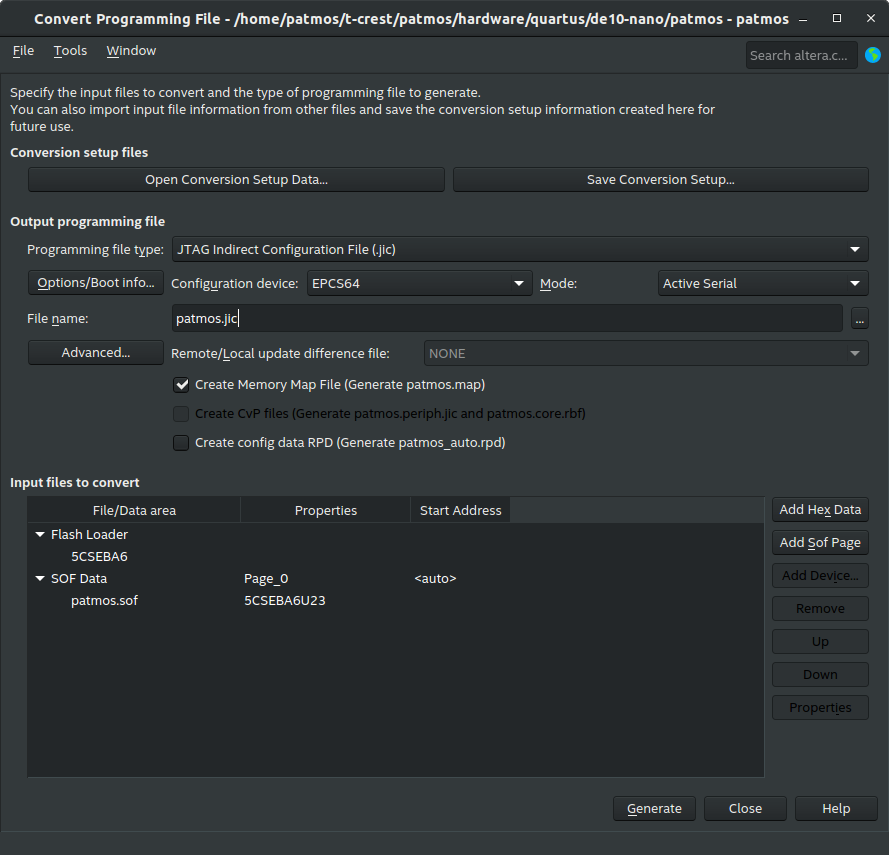
\includegraphics[width=\textwidth]{Figures/setup/quartus_create_jic.png}
    \caption{Convert Programming Files options overview.}\label{fig:app_jic}
\end{figure}    
    
    \item Open the "Program Device" (see the Figure of the Task bar) and it will open a window for downloading the project on the board. Use "Hardware Setup..." to select the DE-SoC port and "Change Files..." to select the .jic project. Notice that it is also necessary to check "Factory default enhanced SFL image".

\begin{figure}[H]
    \centering
        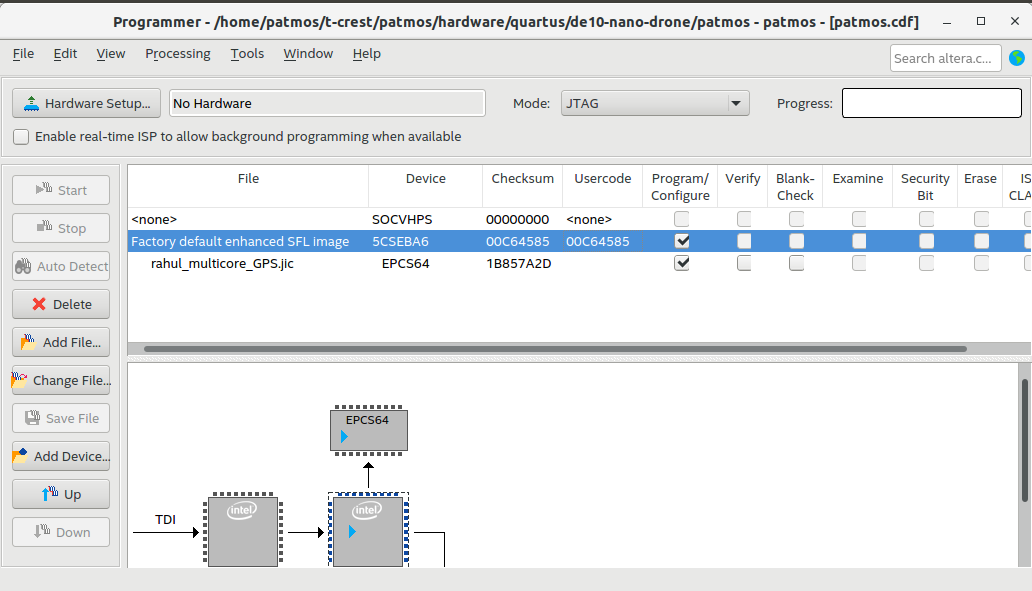
\includegraphics[width=\textwidth]{Figures/setup/quartus_download_jic.png}
    \caption{Download de10-nano-drone project window.}
\end{figure}  
    
    \item After the project is downloaded, re-start the FPGA to be able to download C-apps.

%\end{itemize}
\end{enumerate}

\section*{C apps development through a "Hello World!" tutorial}

This tutorial explains how to create a "Hello World!" C application from scratch and run it on a board.
Before starting, it is necessary to have built and downloaded Patmos as mentioned in the previous sections.  

\begin{enumerate}
    \item Create a folder for the application inside Patmos' app directory. The directory must have the same name as the app.
\lstset{style=Bstyle}
\begin{lstlisting}[language=bash]
cd ~/t-crest/patmos/c/apps && mkdir hello   
\end{lstlisting} 
    \item Create a hello.c file inside the folder with the following content:
\lstset{style=Cstyle}
\begin{lstlisting}
#include <stdio.h>
#include <machine/patmos.h>
#include <machine/spm.h>

int main() {
  printf("Hello wrold!\n");
  return 0;
}      
\end{lstlisting} 
    \item Create a Make file inside the folder, which shall compile the .c file. The \textit{patmos-clang} command transforms the .c main file (and its dependencies) into a binary file compatible with the FPGA. This Makefile contains the following:
\lstset{style=OtherSt}
\lstinputlisting{Figures/setup/Files/Makefile}    
    \item Copy the generated file to the temp directory. This can be done as well inside the Makefile (uncomment last line).
    \item Go back to the main Patmos directory and download the app.
\lstset{style=Bstyle}
\begin{lstlisting}[language=bash]
cd ~/t-crest/patmos/
make APP=hello download
\end{lstlisting} 

\end{enumerate}

\begin{figure}[H]
    \centering
        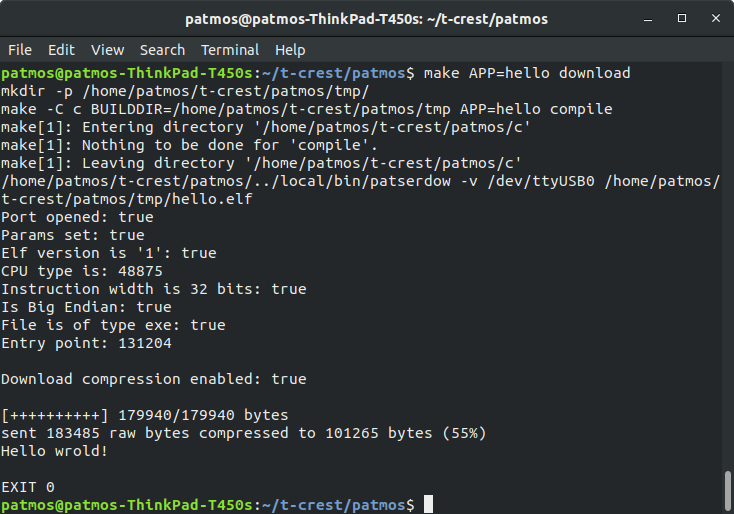
\includegraphics[scale=0.5]{Figures/setup/hello_example.png}
    \caption{Log and result on the terminal after downloading a C app.}
    \label{fig:c_app}
\end{figure}

\section*{Using the Flight Controller}\label{app:sec_fc}

The C-Application for the flight controller and its dependencies are in the \textit{~/t-crest/patmos/} \textit{c/apps/de10-nano/} directory. It contains the main script \textit{Flight\_controller\_2.c} in and the functions for each core are in the header \textit{PREDICTthread.h}. Apart from that, it also contains the following directories:

\begin{itemize}
    \item basic\_lib: contains low-level functions to access the pins and other Patmos-related options (such as counting time, etc). It also contains global variables to access the components and save their outputs, and the additional dependencies for using the GPS and barometer.
    \item FC\_functionalities: contains specific features for flying, such as the PID controller, take off, landing and calibration process.
    \item sensors: contains the handlers and implements the full functionalities for each sensor. These headers use the low-level functions from the basic library to access the sensors data and process it.
    \item sensors\_test: contains a set of different scripts. Each script is meant to be used of a specific single sensor or type of devices.
\end{itemize}
\subsubsection*{Pairing Transmitter and Receiver}\label{trans_receiver_pair}
To pair a transmitter and a receiver:
\begin{enumerate}
    \item Add the binding plug shorting the ground and the signal pins on the receiver.
    \item Power on the receiver and the receiver binding mode is indicated by fast blinking.
    \item Push the bind button on the transmitter and switch it on.
    \item The receiver is bound successfully if it stops blinking.
    \item Now remove the binding plug and the receiver is now paired.
\end{enumerate}

\subsubsection*{Change baud rate of Telemetry}\label{telemetry_baud}
The telemetry modules have to configured to be in the baud rate 115200 using a the software used by the telemetry module \cite{bib:ardupilot} (differs based on the provider of the module). 


\subsubsection*{Tuning the PID gains}
In case the behaviour of the flight controller needs to be tuned, the variables storing the PID gains can be found in the \textit{FC\_global.h} file in the \textit{basic\_lib} folder.

The recommended tuning procedure is described in Section \ref{app:tuning}.

\subsubsection*{Downloading the code}


To download this application on a board:

\begin{itemize}
    \item Select on the Makefile the main script (either the flight controller or one of the test programs available). All the dependencies have been included in this Makefile, do not change something else unless it is necessary.
    
    \lstset{style=Bstyle}
    \begin{lstlisting}[language=bash]
# Uncomment this for using the flight controller
MAIN?=Flight_controller_v2

# Uncomment and/or modify this for running a test program
# MAIN?=sensors_tests/receiver_test

# Modify this if another port is in used
SERIAL?=/dev/ttyUSB0

# Do not modify any further
I2C?=basic_lib/i2c_master
GPS?=basic_lib/gps
LDFLAGS?= \
        -mpatmos-method-cache-size=0x1000 \
        -mpatmos-stack-base=0x080000 -mpatmos-shadow-stack-base=0x078000 \
        -Xgold --defsym -Xgold __heap_end=0x070000

all:
	patmos-clang -I ../.. -O2 $(LDFLAGS) $(I2C).c $(GPS).c $(MAIN).c -o de10-nano.elf -lm
	patmos-clang -I ../.. -O2 $(LDFLAGS) $(I2C).c $(GPS).c $(MAIN).c -o ~/t-crest/patmos/tmp/de10-nano.elf -lm
download:
	patserdow -v $(SERIAL) de10-nano.elf
    \end{lstlisting} 
    
    
    \item Compile the App and download it.
    
\lstset{style=Bstyle}
\begin{lstlisting}[language=bash]
cd ~/t-crest/patmos/c/apps/de10-nano
make
cd ../../..
make APP=de10-nano download
\end{lstlisting} 

\end{itemize} 


\section*{Common troubleshooting}

\begin{itemize}
    \item Sensors and actuators: the different components can be tested individually with their own test programs. In case a specific device seems not to work properly, there are some approaches that you can try:
    \begin{itemize}
        \item In case of using the PCB for attaching the device, review the pins connection with a voltimeter. Follow the hardware diagram and connections shown in Chapter \ref{ch:hw}.
        
        \item In case of not using the PCB and connecting the device directly to the board, review the wiring and power supply. Sometimes it can be that two connections are accidentally switched (TX and RX, or SCL and SDA).
        
        \item Check that the device is not faulty and properly on. In a nutshell: IMU must light green, the barometer GPS+compass light red, the telemetry lights permanently green and the receiver red.
        
        In case the telemetry module is blinking green, it means it cannot reach its paired module, so it is necessary to review the connection between modules.If it permanently red is on configuration status, which means it needs to be connected to a computer with SikRadio \cite{bib:ardupilot} and its firmware needs to be re-uploaded. 
        
        In case the receiver is blinking-slow red, it means it cannot reach its paired transmitter, so review that the transmitter is properly on and paired to it. In case the receiver is blinking-fast red, it is on pairing mode and it needs to be paired with a transmitter and restarted afterwards, see Section \ref{app:sec_fc}.
        
        \item In case the device seems to be working fine, it could be that it is assigned to the wrong core or with the wrong settings. Review the hardware settings on the \textit{de10-nano-drone.xml}.
        
        Then modify Patmos configuration to single-core and with all the devices assigned to core 0. Then change the test program to one single thread with the function for that specific device.
    \end{itemize}
    
    \item Compiling Patmos: a server compiles and builds Patmos periodically to verify it is properly set, so it should not be a problem to build it and compile in a laptop.
    
    In case of compiling Patmos when it has been updated after some time, update not just the patmos repository, but all the repositories from the t-crest folder. Then follow the presented instructions for downloading Patmos on the board. Most of the building issues come from Step 4, where the libraries are built, so try to run the $./build.sh$ from another directory or rebuilding the newlib by steps.
    
    Also review that the board model is correctly specified as $de10-nano-drone$.
    
    \item Downloading Patmos: for this specific the project, the Patmos architecture is multicore, so review first the microSD card is correctly flashed and inserted. For this project the microSD cards were flashed in a Windows computer using Windiskimager32.
    
    Review afterwards the settings for the .jic file in Figure \ref{fig:app_jic} and remember to re-start the FPGA.
    
    \item Compiling C apps: use the Patmos dependencies libraries as presented in this project and other Patmos-app examples. 
    
    Also before downloading an app, review that the generated .elf files from the C code are updated. There is a difference between compiling an App from its own folder (it generates an .elf file there) than from Patmos main directory (it generates an .elf file on the $~/t-crest/patmos/tmp$ directory), so it can be that an App is built differently depending on the process and it can also be that the .elf file downloaded on the board is outdated. 
    
    For this project, the flight controller application was built on its own folder and the Makefile would create the two .elf files.
    
    
    \item Downloading C apps: here are some of the most common issues:
\lstset{style=Bstyle}
\begin{lstlisting}[language=bash]
java.util.concurrent.TimeoutException: Receiver did not reply (715 responses missing)
jssc.SerialPortException: Port name - /dev/ttyUSB0; Method name - openPort(); Exception type - Permission denied.
\end{lstlisting} 

Review that the user account has root privileges on the ports communication, on the steps 1 and 2 from downloading Patmos.
    
\lstset{style=Bstyle}
\begin{lstlisting}[language=bash]
java.util.concurrent.TimeoutException: Receiver did not reply (715 responses missing)
jssc.SerialPortException: Port name - /dev/ttyUSB0; Method name - closePort(); Exception type - Port not opened.
\end{lstlisting} 

Review that the FPGA drivers are properly installed and that not other process has not already access the port. Sometimes the easiest way is to disconnect the FPGA, re-start it and connect it again.

\lstset{style=Bstyle}
\begin{lstlisting}[language=bash]
java.util.concurrent.TimeoutException: Receiver did not reply (715 responses missing)
jssc.SerialPortException: Port name - /dev/ttyUSB0; Method name - openPort(); Exception type - Port not found.
\end{lstlisting} 

Review that UART-USB port is properly powered up (the drone should have the battery connected) and the port number matches what it is specified on the Makefile from $~/t-crest/patmos$.
    
\end{itemize}
% ===================================================================================
% Add this chapter to the table of contents:
%\addcontentsline{toc}{chapter}{Appendix: how to set up the drone}
